\section{RISMC Approach to PRA}
\label{sec:rismc}

The RISMC approach~\cite{RISMC} employs both deterministic and stochastic methods 
in a single analysis framework (see Figure~\ref{fig:RISMCoverview}). In the deterministic method 
set we include:
\begin{itemize}
  \item Modeling of the thermal-hydraulic behavior of the plant~\cite{BWR_SBO_Mandelli,BWRanalysis}
  \item Modeling of external events such as flooding~\cite{mandelliPSA2015}
  \item Modeling of the operators’ responses to the accident scenario~\cite{HRA_BoringReport2014}
\end{itemize}

\begin{figure}
    \centering
    \centerline{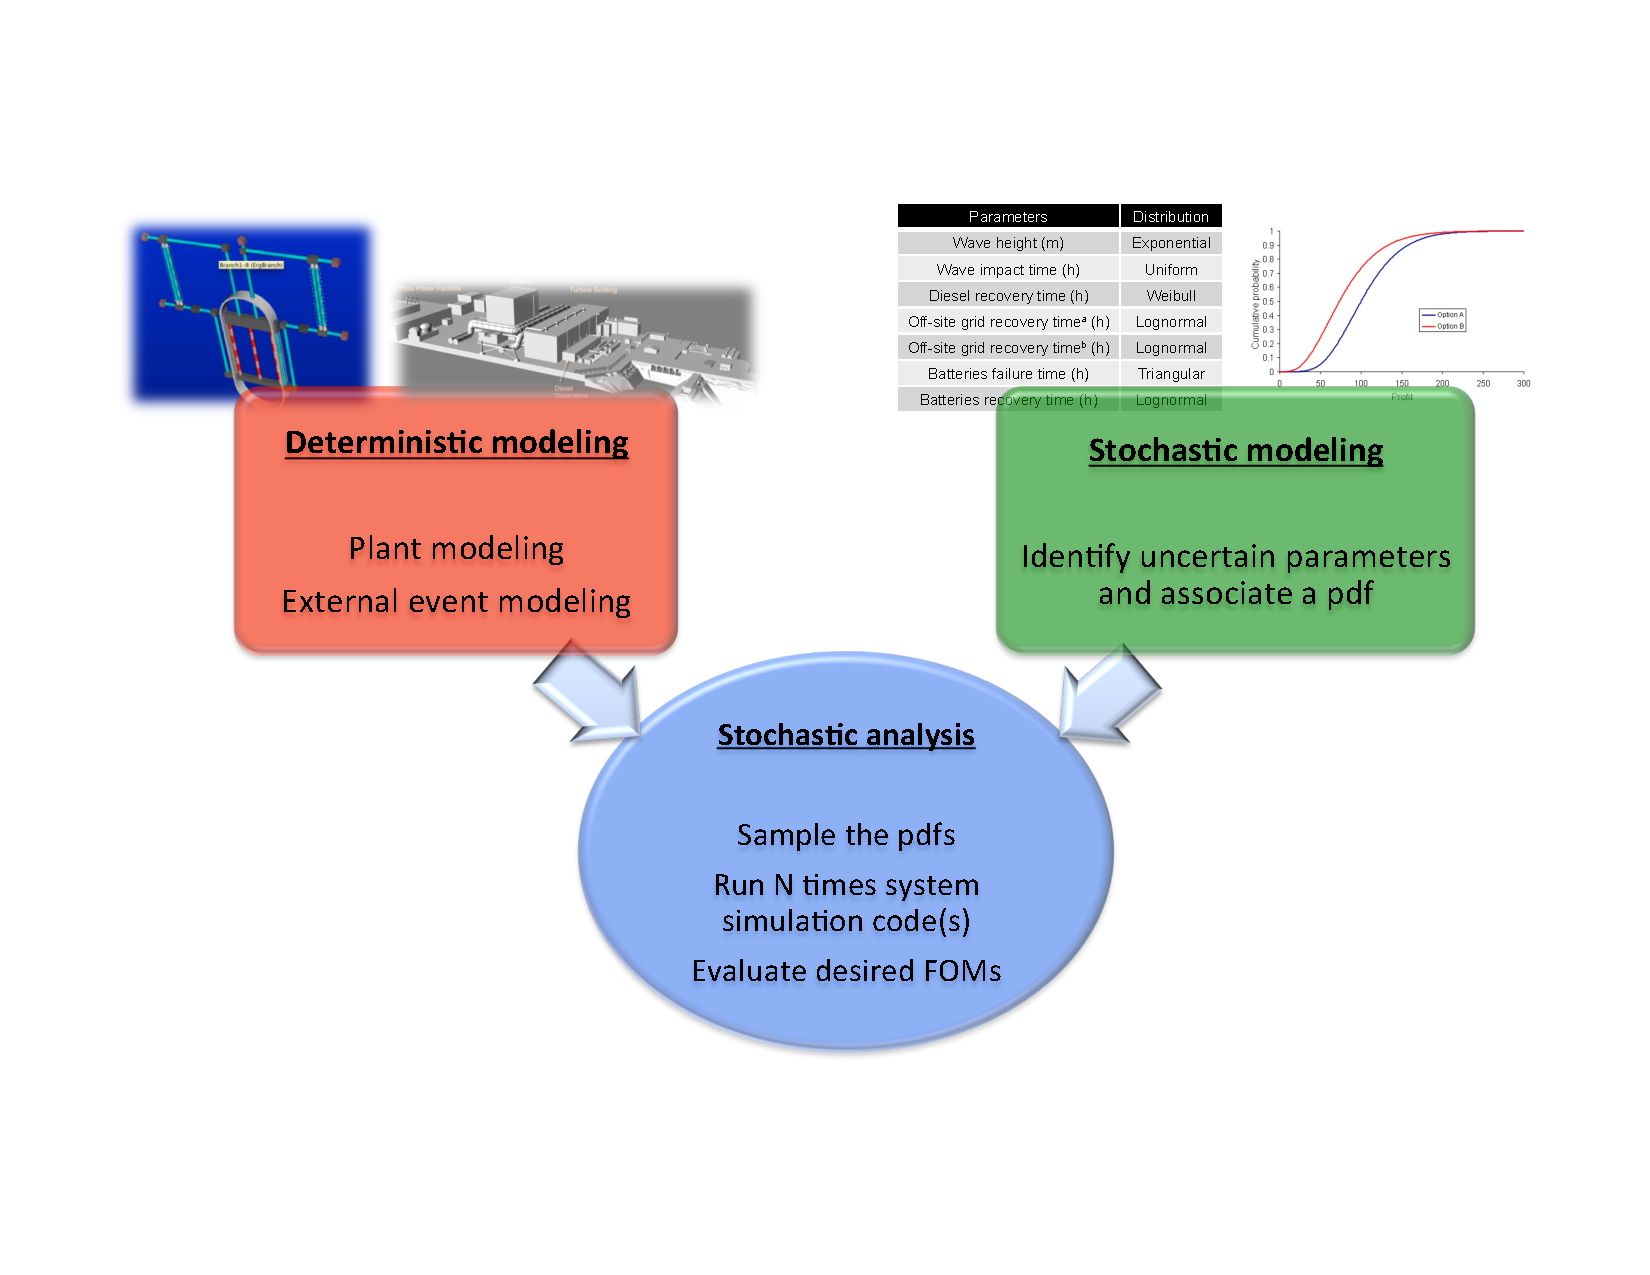
\includegraphics[scale=0.4]{RISMCoverview.pdf}}
    \caption{Overview of the RISMC approach}
    \label{fig:RISMCoverview}
\end{figure}

Note that deterministic modeling of the plant or external events can be performed by employing specific 
simulator codes but also surrogate models~\cite{ROM}, known as reduced order models (ROM). ROMs would 
be employed 
in order to decrease the high computational costs of employed codes. In addition, multi-fidelity codes 
can be employed to model the same system; the idea is to switch from low-fidelity to high-fidelity code 
when higher accuracy is needed (e.g., use low-fidelity codes for steady-state conditions and high-fidelity 
code for transient conditions)

In the stochastic modeling we include all stochastic parameters that are of interest in the PRA analysis 
such as uncertain parameters and stochastic failure of system/components.
As mentioned earlier, the RISMC approach heavily relies on multi-physics system simulator codes 
(e.g., RELAP5-3D~\cite{relap5}) coupled with stochastic analysis tools (e.g., RAVEN~\cite{raven}).  
From a PRA point of view, this type of simulation can be described by using two sets of variables:
\begin{itemize}
  \item $\boldsymbol c = \boldsymbol c(t)$ represents the status of components and systems of the simulator 
        (e.g., status of emergency core cooling system, AC system)
  \item $\boldsymbol \theta = \boldsymbol \theta (t)$ represents the temporal evolution of a simulated 
        accident scenario, i.e., $\boldsymbol \theta (t)$ represents a single simulation run. 
        Each element of $\boldsymbol \theta$ can be for example the values of temperature or pressure in 
        a specific node of the simulator nodalization.
\end{itemize}

From a mathematical point of view, a single simulator run can be represented as a single trajectory in the 
phase space. The evolution of such a trajectory in the phase space can be described as follows:
\begin{equation}
  \begin{cases}
    \dfrac{\partial \boldsymbol \theta }{\partial t}  = \boldsymbol \Xi (\boldsymbol \theta , \boldsymbol c, \boldsymbol s , t)   \\ \\ 
    \dfrac{\partial \boldsymbol c }{\partial t}  = \boldsymbol \Gamma (\boldsymbol \theta , \boldsymbol c, \boldsymbol s , t) 
  \end{cases}    
  \label{eq:trajectory}
\end{equation}
where:
\begin{itemize}
  \item $\boldsymbol \Xi$ is the actual simulator code that describes how θ evolves in time
  \item $\boldsymbol \Gamma$ is the operator which describes how c evolves in time , i.e., the status 
        of components and systems at each time step
  \item $\boldsymbol C$ is the set of stochastic parameters.
\end{itemize}

Starting from the system located in an initial state, $\boldsymbol \theta (t=0) = \boldsymbol \theta(0)$, 
and the set of stochastic parameters (which are generally generated through a stochastic sampling process), 
the simulator determine at each 
time step the temporal evolution of $\boldsymbol \theta (t)$. At the same time, the system control logic  
determines the status of the system and components $\boldsymbol c(t)$.
 
By using the RISMC approach, the PRA analysis is performed by~\cite{}:
\begin{enumerate}
  \item Associating a probabilistic distribution function (pdf) to the set of parameters 
        $\boldsymbol s$ (e.g., timing of events)
  \item Performing stochastic sampling of the pdfs defined in Step 1
  \item Performing a simulation run given $\boldsymbol s$ sampled in Step 2, i.e., solve the 
        system of equations~\ref{??}
  \item Repeating Steps 2 and 3 $M$ times and evaluating user defined stochastic parameters such 
        as core damage (CD) probability ($P_{CD}$).
\end{enumerate}

\subsection{RISMC Approach and Classical PRA}
\label{sec:analogy}

In order to better understand the results obtained in Section~\ref{sec:test} it is worth to illustrate 
a link between classical PRA and RISMC approach.
Let's consider a system that is composed by two components (i.e, A and B) in a series configuration where
each component has a failure probability (i.e., $p_A$ and $p_B$ respectively) as shown in Fig.~\ref{fig:ABsystem}.

In a classical PRA framework such system can be modeled using a FT method that is composed by two basic events:
A failed and B failed.
System failure would be represented by a single ``AND'' gate that combine the two basic events as shown in 
Fig.~\ref{fig:ABsystem}.

In a RISMC approach, such system would be modeled by using two stochastic parameters (i.e., $var_A$ and $var_B$)
with a Bernoulli distribution $\operatorname{Bern}(p)$ associated to each of them: 
$var_A \sim \operatorname{Bern}(p_A)$ and $var_B \sim \operatorname{Bern}(p_B)$. 
The model that emulates system response would simply implement the ``AND" logic of the $var_A$ and $var_B$. 
In order to determine system failure probability a numerical integration has to be performed in a 2-dimensional 
(a dimension for each stochastic parameter).

Two possible sampling strategies can be followed:
\begin{itemize}
  \item Monte-Carlo: generate $N$ samples and count the the number of samples that lead to system failure
  \item Grid: partition the 2-dimensional space into a Cartesian grid; generate a sample for each partition 
        and associate a probability weight $w$ to each sample. This weight can be determined by integrating the pdf
        $pdf(A,B) = B(p_A) B(p_B)$ in each partition. In this specific case, since each stochastic parameter 
        has two possible outcomes (i.e. 0 and 1), the space has been partitioned into 4 regions as 
        shown in Fig.~\ref{fig:2Danalogy}. Each cell of Fig.~\ref{fig:2Danalogy} has indicated the system outcome:
        system failure (F) or system success (OK).
\end{itemize}

The Monte-Carlo would require a large number of samples in order to decrease the statistical error associated
to system failure probability.
On the other hand a Grid sampler would determine the exact value of system failure probability with only 4 samples:
\begin{enumerate}
  \item sample 1: $A=0$ and $B=0$ (bottom left cell of Fig.~\ref{fig:2Danalogy}), $w_1 = (1-p_A)(1-p_B)$
  \item sample 2: $A=1$ and $B=0$ (top left cell of Fig.~\ref{fig:2Danalogy}), $w_2 = p_A (1-p_B)$
  \item sample 3: $A=0$ and $B=1$ (bottom right cell of Fig.~\ref{fig:2Danalogy}), $w_3 = (1-p_A) p_B$
  \item sample 4: $A=1$ and $B=1$ (top right cell of Fig.~\ref{fig:2Danalogy}), $w_4 = p_A p_B$
\end{enumerate}
Note that each sample/cell of Fig.~\ref{fig:2Danalogy} that leads to system failure corresponds to a specific cut-set
\begin{itemize}
  \item Cut-set 1 (CS1) corresponds to sample 2; $p_{CS1} = p_A$
  \item Cut-set 2 (CS2) corresponds to sample 3; $p_{CS2} = p_B$
  \item Cut-set 3 (CS3) corresponds to sample 4; $p_{CS3} = p_A p_B$
\end{itemize}
Hence, the two methods (classical and PRA) would provide identical results.

Observe now that the number of samples required for $M$ stochastic parameters (assuming they are all distributed with 
a Bernoulli distribution) would be equal to $2^M$. Thus this strategy can be employed for a small value of $M$.


\begin{figure}
  \centering
  \begin{subfigure}{.5\textwidth}
    \centering
    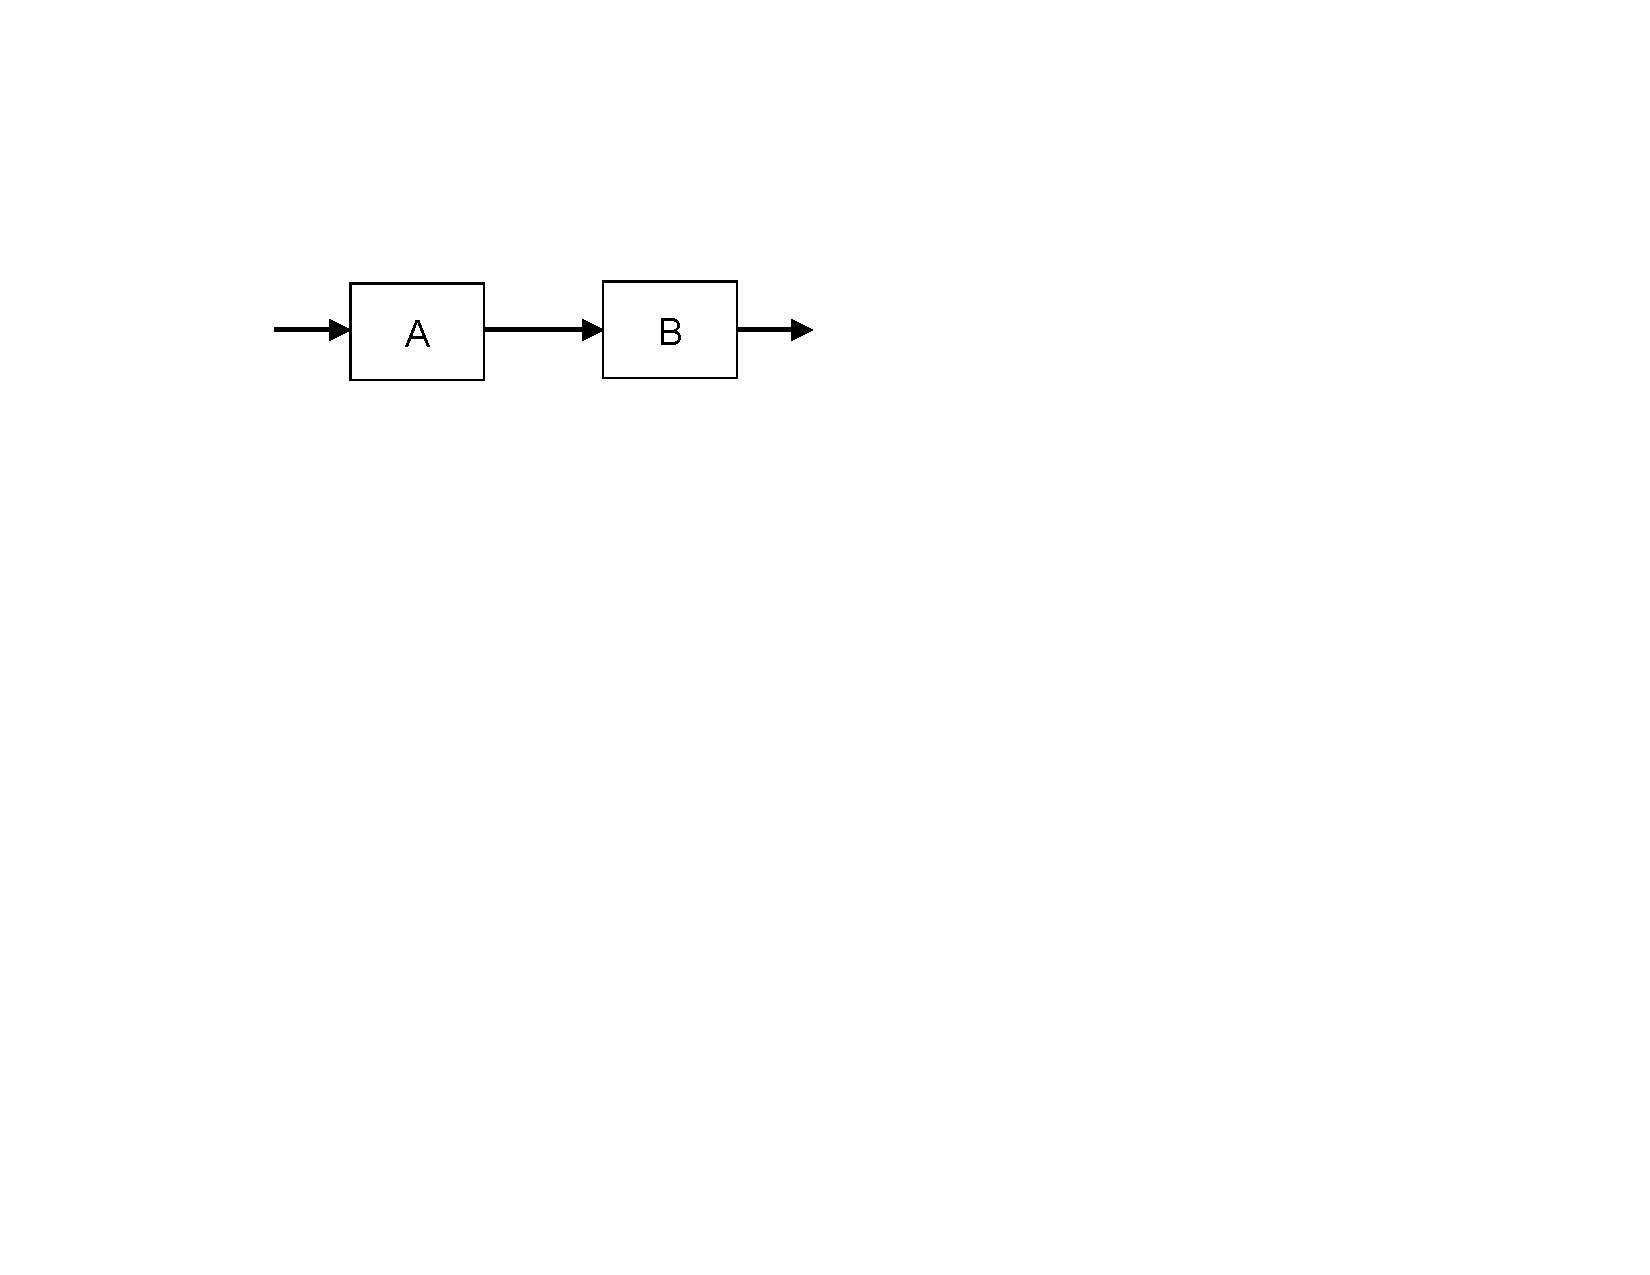
\includegraphics[scale=0.6]{ABsystem.pdf}
    \label{fig:sub1}
  \end{subfigure}%
  \begin{subfigure}{.5\textwidth}
    \centering
    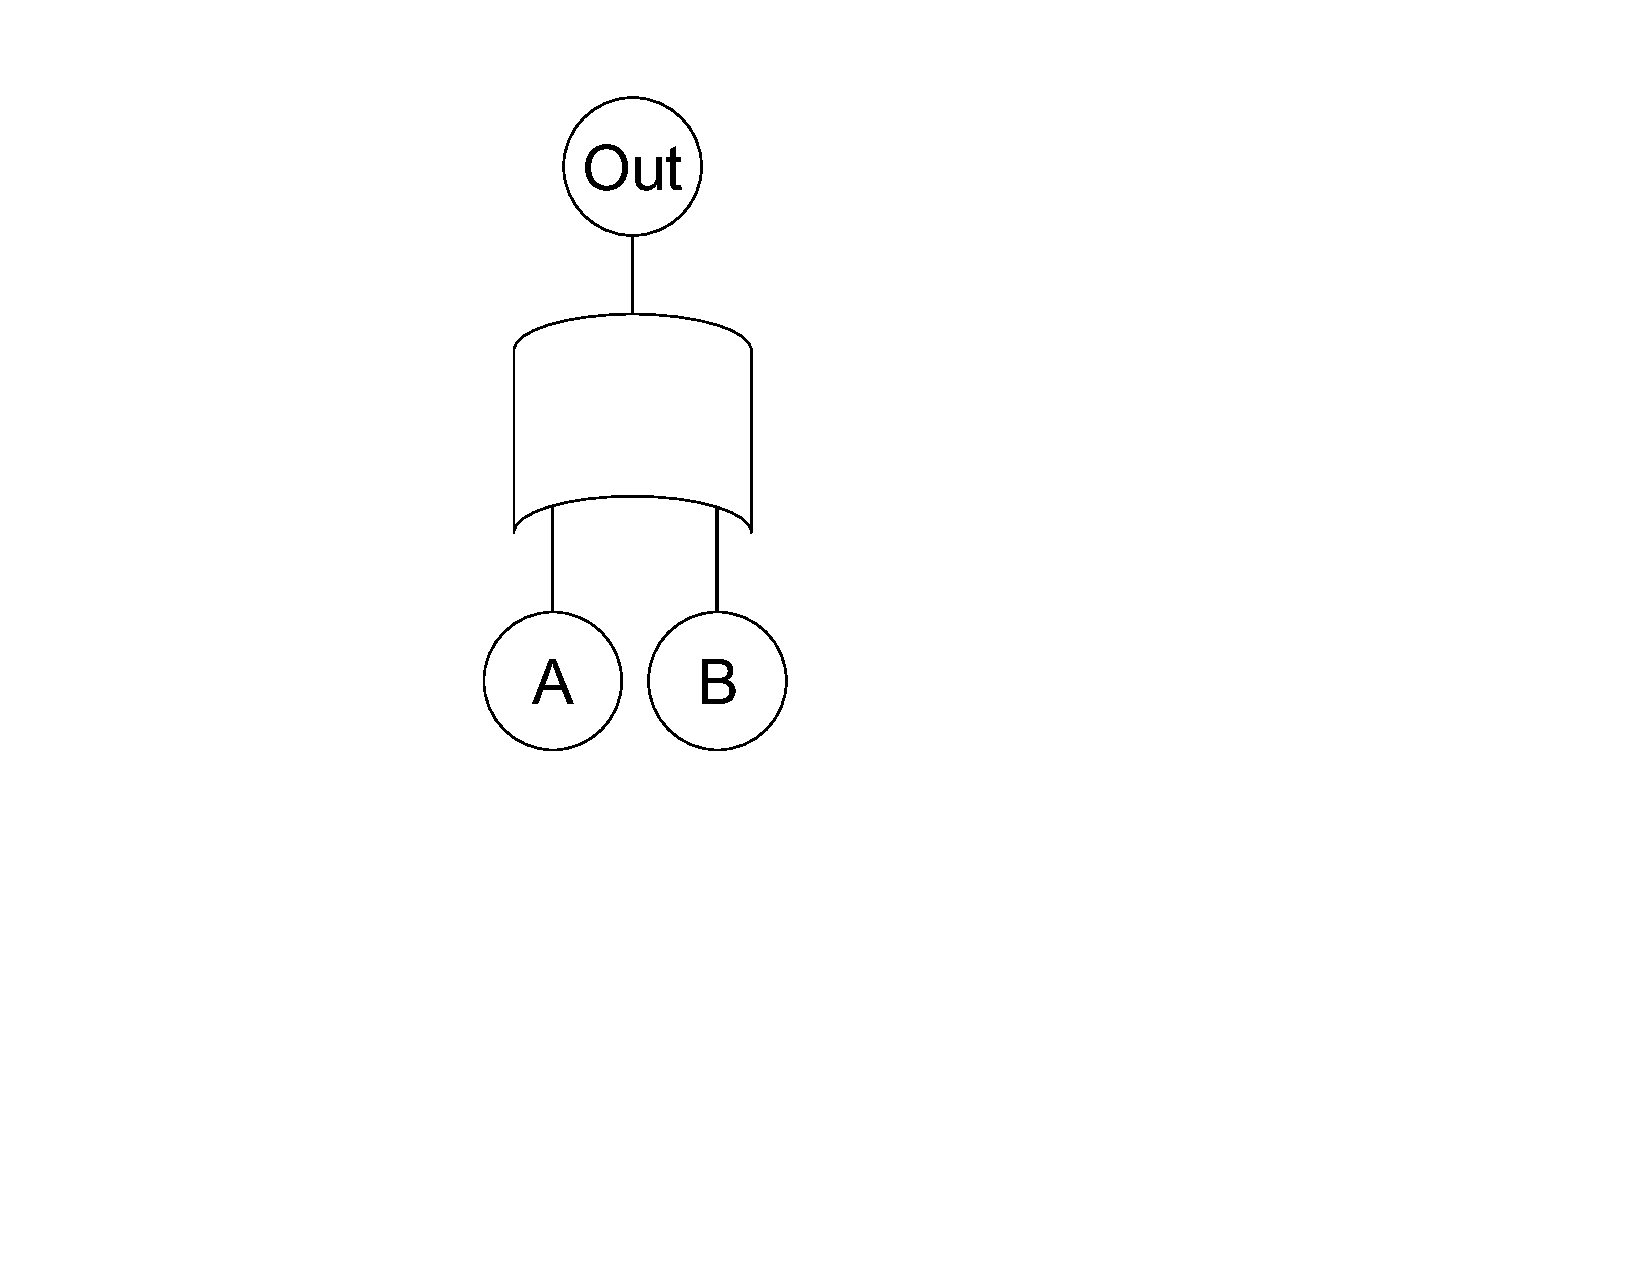
\includegraphics[scale=0.3]{andGate.pdf}
    \label{fig:sub2}
  \end{subfigure}
  \caption{Components A and B in a series configuration (left) and its associated Fault-Tree (right).}
  \label{fig:ABsystem}
\end{figure}

\begin{figure}
    \centering
    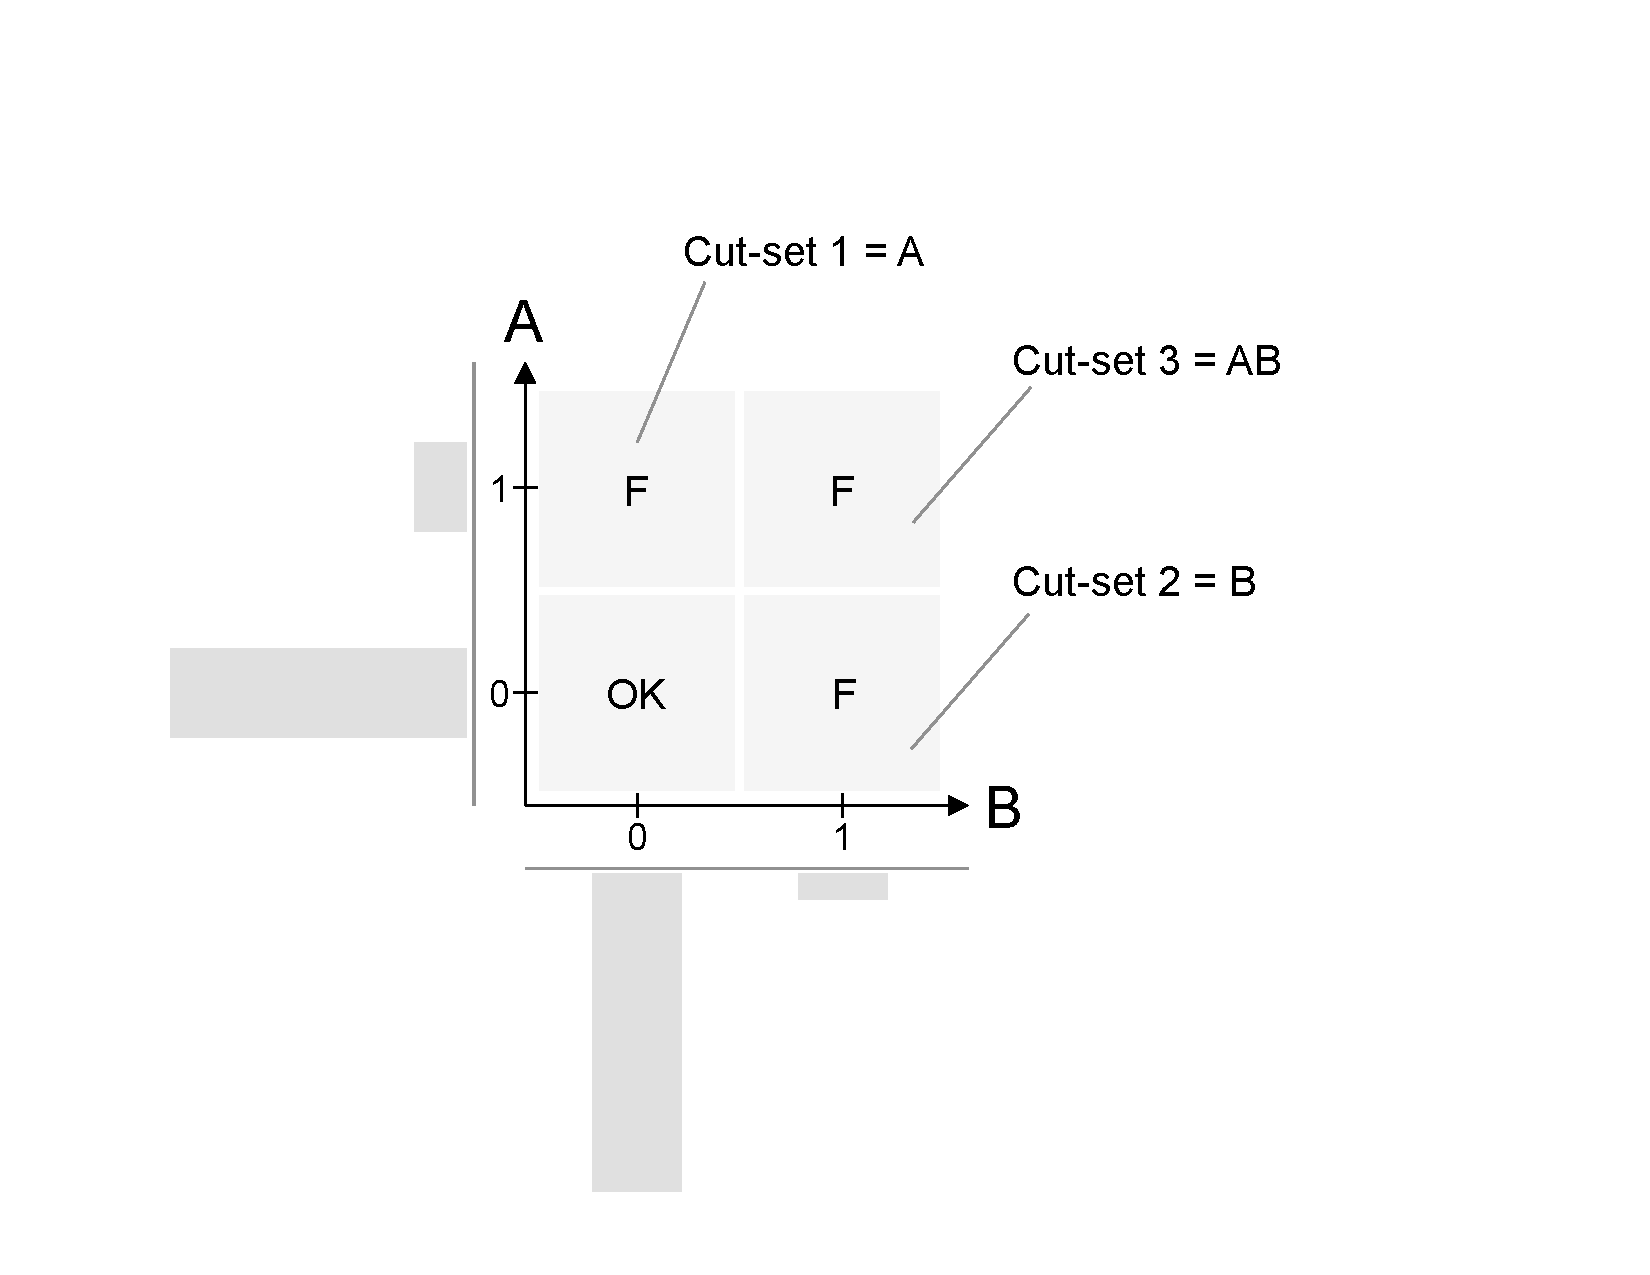
\includegraphics[scale=0.4]{2D.pdf}
    \caption{}
    \label{fig:2Danalogy}
\end{figure} 



